\documentclass[11pt]{article}
\usepackage[margin=1in]{geometry}
\usepackage[T1]{fontenc}
\usepackage[utf8]{inputenc}
\usepackage{lmodern}
\usepackage{microtype}
\usepackage{amsmath,amssymb}
\usepackage{booktabs,tabularx,array}
\usepackage{graphicx}
\usepackage{xcolor}
\usepackage{enumitem}
\usepackage{hyperref}
\usepackage{caption}
\usepackage{tikz}
\usetikzlibrary{positioning,arrows.meta,shapes.misc,fit,backgrounds}
\hypersetup{colorlinks=true,linkcolor=blue!60!black,citecolor=blue!60!black,urlcolor=blue!60!black}
\captionsetup{font=small,labelfont=bf}
\setlist[itemize]{leftmargin=1.4em,topsep=3pt,itemsep=2pt,parsep=0pt}
\setlength{\parskip}{0.45em}
\setlength{\parindent}{0pt}
\setlength{\textfloatsep}{12pt plus 2pt minus 2pt}
\newcommand{\method}{\textsc{DotCache}}
\newcommand{\kv}{KV}
\newcommand{\kvc}{\kv cache}
\newcommand{\todo}[1]{\textcolor{red}{#1}}

\title{\vspace{-1.2em}\method: Executing Attention Directly on Compressed \kv{} Caches}
\author{Anonymous Draft\\\small Replace with author names and affiliations before submission}
\date{March 2026}

\begin{document}
\maketitle

\begin{abstract}
Long-context LLM inference is increasingly constrained by \kv{} memory footprint and bandwidth rather than raw matrix throughput. Recent work has made aggressive \kv{} compression plausible: KVQuant, KIVI, QJL, PolarQuant, TurboQuant, and InnerQ all show that 2--4 bit key-value representations can preserve model quality under realistic workloads \cite{kvquant,kivi,qjl,polarquant,turboquant,innerq}. Yet most serving stacks still treat quantized \kv{} as a storage format that must be widened before attention executes, leaving dequantization overhead and intermediate traffic on the critical path \cite{qserve,innerq}. This paper argues for a different abstraction: low-bit \kv{} should be treated as an \emph{execution format}. We propose \method{}, a compressed-domain \kv{} substrate that stores page-organized low-bit keys and values with compact metadata and fuses symbol unpacking, lightweight decode, and attention computation into a single datapath. \method{} supports asymmetric key and value codecs, optional structured preconditioning on the write path, and per-head adaptive modes. This paper is intentionally a systems proposal rather than a benchmark paper: it defines the architecture, software contract, cost model, and evaluation plan for a hardware-native next step in long-context inference. The central claim is simple: once sub-4-bit \kv{} is credible, the next bottleneck is no longer only codec quality, but where decode happens and how much data is widened on the way to attention.
\end{abstract}

\section{Introduction}

As context windows grow from tens of thousands of tokens toward million-token regimes, autoregressive LLM serving becomes increasingly memory-bound. The reason is familiar: the \kvc{} scales linearly with sequence length, and every decode step must repeatedly revisit historical keys and values. Recent surveys frame \kv{} management as a first-class systems problem because it affects memory footprint, bandwidth consumption, and latency at the same time \cite{kvcachesurvey}. The serving literature makes the same point from a runtime perspective. PagedAttention and vLLM showed that better \kv{} memory organization can deliver large throughput gains even without changing the underlying model \cite{pagedattention}. XQuant goes further and argues that modern hardware trends already favor trading more compute for fewer memory operations \cite{xquant}.

At the same time, the algorithmic picture has changed quickly. KVQuant reports sub-4-bit \kv{} quantization with negligible perplexity degradation and custom CUDA kernels \cite{kvquant}. KIVI shows that keys and values benefit from different grouping strategies, with per-channel quantization for keys and per-token quantization for values \cite{kivi}. QJL eliminates explicit scale-and-zero-point metadata through a quantized Johnson-Lindenstrauss transform \cite{qjl}. PolarQuant and TurboQuant exploit transformed coordinates and distributional structure to make extremely low-bit \kv{} compression practical \cite{polarquant,turboquant}. InnerQ makes an explicitly hardware-aware point: grouping along the inner dimension of the vector-matrix product can reduce dequantization overhead and improve end-to-end decode latency \cite{innerq}.

Those results collectively change the design space. The main question is no longer whether low-bit \kv{} is possible. It is whether inference systems should continue to treat low-bit \kv{} as compressed bytes at rest that must be expanded before attention runs. QServe reports that dequantization overhead can consume 20--90\% of runtime in low-bit serving pipelines \cite{qserve}. InnerQ reaches a similar conclusion from a different angle: layout and grouping strategy matter because dequantization and score computation are tightly coupled in practice \cite{innerq}. In other words, codec quality and execution strategy can no longer be separated cleanly.

This paper proposes \method{}, a compressed-domain \kv{} execution substrate for long-context LLM inference. \method{} is not a new quantizer. Instead, it is an architectural proposal for how the attention path should consume already-compressed \kv{} data. The core idea is to move decode as close as possible to the final multiply-accumulate, and to avoid fully materializing dequantized key or value tensors unless a fallback path demands it.

\textbf{Contributions.} This paper makes four contributions:
\begin{itemize}
    \item It reframes low-bit \kv{} from a storage optimization into an execution abstraction for attention.
    \item It defines a page-oriented compressed-domain pipeline with fused \emph{decode-score} and \emph{decode-mix} stages.
    \item It proposes a codec-agnostic software contract that can host affine, LUT-based, sketch-based, and transformed-coordinate \kv{} codecs.
    \item It outlines a practitioner-oriented prototype and evaluation plan, so the idea can be tested in GPU kernels before any hardware specialization exists.
\end{itemize}

\section{Why storage-only \kv{} compression leaves performance on the table}

Low-bit \kv{} compression only helps end-to-end inference if the saved bytes outweigh three hidden costs: metadata fetches, decode work, and widening traffic. This section makes the open gap concrete.

\subsection{Compression ratio is not the whole story}

Most low-bit \kv{} papers optimize a storage or distortion objective. That is necessary, but it is not sufficient for runtime wins. A nominal 3-bit or 4-bit format can still disappoint if the system must fetch scale tables, unpack symbols into wide registers, reconstruct FP16 intermediates, and only then compute attention. QServe shows exactly this pathology for low-bit serving more broadly: explicit dequantization can become a dominant overhead on GPUs \cite{qserve}. InnerQ makes the same point specifically for \kv{} quantization, arguing that grouping over the inner dimension is attractive because it aligns the quantization layout with the vector-matrix multiplication and reduces redundant memory accesses \cite{innerq}.

\subsection{Current runtimes mostly compress for storage, not execution}

Existing methods contribute important pieces of the solution, but most still stop short of a full compressed-domain execution abstraction:
\begin{itemize}
    \item \textbf{PagedAttention} organizes \kv{} blocks efficiently in memory, but the abstraction is still a block of conventional tensors rather than an execution-native code stream \cite{pagedattention}.
    \item \textbf{KVQuant}, \textbf{KIVI}, \textbf{QJL}, \textbf{PolarQuant}, and \textbf{TurboQuant} show that low-bit \kv{} representations can be accurate and memory efficient, but they do not define a common substrate for fused decode and attention execution \cite{kvquant,kivi,qjl,polarquant,turboquant}.
    \item \textbf{QServe} and \textbf{InnerQ} reveal where low-bit systems lose time in practice, which motivates a more execution-aware design \cite{qserve,innerq}.
    \item \textbf{PQCache} and \textbf{XQuant} expose adjacent alternatives on the same frontier: retrieval-first filtering and activation rematerialization, respectively \cite{pqcache,xquant}.
\end{itemize}

\subsection{The missing abstraction}

The missing layer is an explicit distinction between a \emph{storage format} and an \emph{execution format}. A storage format answers the question: ``How can I fit more \kv{} into memory?'' An execution format answers the stronger question: ``How can the attention kernel consume those codes directly, with minimal widening and minimal metadata traffic?''

That distinction matters because keys and values are consumed differently. Keys feed inner products with the current query. Values feed weighted accumulation after softmax. The ideal codec, layout, and precision regime need not be identical for those two paths. KIVI already hints at this asymmetry at the quantization level \cite{kivi}. \method{} generalizes it into an execution model.

\section{The \method{} design}

\subsection{Design principles}

\method{} is built around five design principles.

\textbf{P1. Low-bit \kv{} should be an execution format.} The default path should not reconstruct full FP16/BF16 tensors before attention.

\textbf{P2. Keys and values deserve asymmetric treatment.} Key scoring is an inner-product problem; value mixing is a weighted accumulation problem. A shared bitwidth does not imply a shared best codec.

\textbf{P3. Metadata must be amortized aggressively.} Compression wins disappear quickly if every small block carries expensive side information.

\textbf{P4. Scheduling should be page-granular.} The serving abstraction should be a small, fetchable page indexed by layer, head, token range, and tensor type. This aligns naturally with paged runtimes such as vLLM \cite{pagedattention}.

\textbf{P5. Adaptivity should remain online.} A practical serving stack should allow per-layer, per-head, and age-dependent mode selection without retraining the base model.

\subsection{Data layout}

A \method{} page is indexed by
\[
(\ell, h, t_0{:}t_1, \tau), \qquad \tau \in \{K, V\},
\]
where $\ell$ is the layer, $h$ is the attention head, $t_0{:}t_1$ is a token range, and $\tau$ identifies whether the page stores keys or values. Within a page, vectors are partitioned into fixed-width groups along the inner dimension, for example 32 or 64 channels.

Each group is encoded using one of a small number of modes:
\begin{itemize}
    \item \textbf{M0:} affine low-bit quantization with shared scale and bias,
    \item \textbf{M1:} nonuniform low-bit LUT quantization,
    \item \textbf{M2:} sketch-plus-residual mode for inner-product-aware key execution,
    \item \textbf{M3:} high-precision escape mode for exceptions or a recent-token window.
\end{itemize}

A compact page header stores mode identifiers, shared parameters, optional exception bitmaps, and a small amount of scheduler metadata. The goal is not to invent a universal codec. The goal is to define a common envelope that existing codecs can target.

\subsection{Execution model}

The read and write paths are intentionally asymmetric.

\paragraph{Write path.} Newly produced key and value vectors may optionally pass through a structured preconditioning transform. This can be as simple as a lightweight normalization or as ambitious as a random rotation used by PolarQuant or TurboQuant-style pipelines \cite{polarquant,turboquant}. The transformed vectors are partitioned into inner-dimension groups, encoded according to their selected modes, packed into bitstreams, and written into page-organized \kvc{} storage.

\paragraph{Read path for keys.} When a new query attends over historical context, the runtime fetches compressed key pages rather than full-precision key tensors. Page headers are decoded into fast memory, symbols are unpacked into execution lanes, and score computation proceeds through a fused decode-and-dot-product pipeline. Let $q_g$ denote the slice of the current query corresponding to group $g$, and let $c_{j,g}$ denote the compressed code stream for token $j$ and group $g$. Then the score for token $j$ is computed as
\[
 s_j \approx \sum_g q_g^\top D_K(c_{j,g}, m_g),
\]
where $D_K(\cdot)$ is the key-side decode primitive parameterized by metadata $m_g$. The central implementation rule is that $D_K$ should feed multiply-accumulate units directly, without materializing a wide intermediate unless the runtime falls back to an escape mode.

\paragraph{Read path for values.} After softmax yields weights $\alpha_j$, value pages are fetched and consumed through a fused decode-and-accumulate path:
\[
 o \leftarrow o + \sum_j \alpha_j D_V(c^{V}_{j,g}, m^{V}_g).
\]
Again, values are not reconstructed into a full FP16 matrix by default. The output accumulator is the first wide representation on the main path.

\begin{figure}[t]
\centering
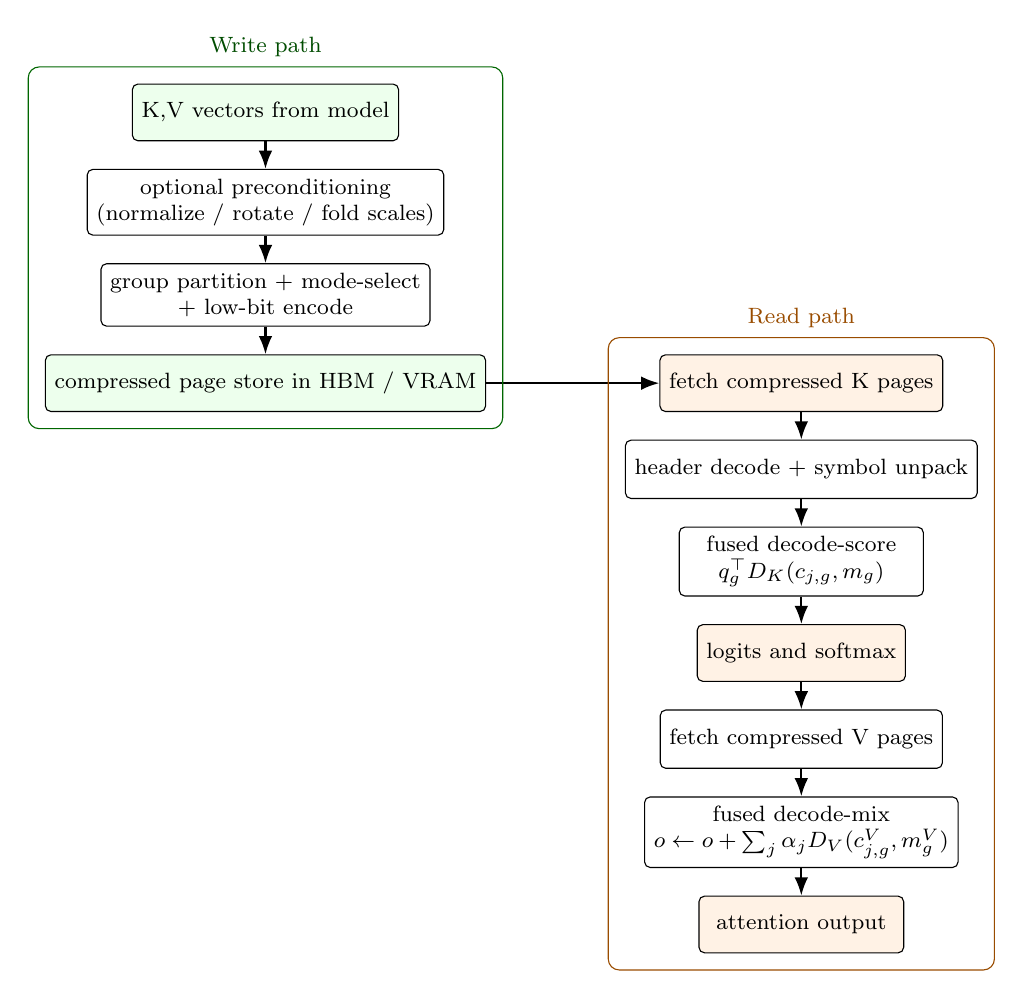
\begin{tikzpicture}[
    font=\footnotesize,
    box/.style={draw, rounded corners=2pt, align=center, minimum width=2.6cm, minimum height=0.72cm, fill=blue!4},
    stage/.style={draw, rounded corners=2pt, align=center, minimum width=3.1cm, minimum height=0.74cm, fill=white},
    arr/.style={-Latex, thick},
    node distance=3.5mm,
]

\node[box, fill=green!7] (kvin) {K,V vectors from model};
\node[stage, below=of kvin] (prep) {optional preconditioning\\(normalize / rotate / fold scales)};
\node[stage, below=of prep] (encode) {group partition + mode-select\\+ low-bit encode};
\node[box, below=of encode, fill=green!7] (store) {compressed page store in HBM / VRAM};

\node[box, right=2.2cm of store, fill=orange!10] (fetchk) {fetch compressed K pages};
\node[stage, below=of fetchk] (headerk) {header decode + symbol unpack};
\node[stage, below=of headerk] (score) {fused decode-score\\$q_g^\top D_K(c_{j,g}, m_g)$};
\node[box, below=of score, fill=orange!10] (softmax) {logits and softmax};
\node[stage, below=of softmax] (fetchv) {fetch compressed V pages};
\node[stage, below=of fetchv] (mix) {fused decode-mix\\$o \leftarrow o + \sum_j \alpha_j D_V(c^V_{j,g}, m_g^V)$};
\node[box, below=of mix, fill=orange!10] (out) {attention output};

\draw[arr] (kvin) -- (prep);
\draw[arr] (prep) -- (encode);
\draw[arr] (encode) -- (store);
\draw[arr] (store.east) -- ++(0.9,0) |- (fetchk.west);
\draw[arr] (fetchk) -- (headerk);
\draw[arr] (headerk) -- (score);
\draw[arr] (score) -- (softmax);
\draw[arr] (softmax) -- (fetchv);
\draw[arr] (fetchv) -- (mix);
\draw[arr] (mix) -- (out);

\node[draw=green!40!black, rounded corners=4pt, fit=(kvin)(prep)(encode)(store), inner sep=6pt, label={[green!30!black]above:Write path}] {};
\node[draw=orange!60!black, rounded corners=4pt, fit=(fetchk)(headerk)(score)(softmax)(fetchv)(mix)(out), inner sep=6pt, label={[orange!60!black]above:Read path}] {};
\end{tikzpicture}
\caption{\method{} treats compressed \kv{} as an execution format. The write path encodes page-organized low-bit representations; the read path fuses unpacking, lightweight decode, and attention computation so keys and values are not widened into full tensors by default.}
\label{fig:pipeline}
\end{figure}

\subsection{Hardware mapping}

A hardware-conscious \method{} implementation naturally decomposes into five blocks.

\textbf{Page fetch and prefetch.} A page unit fetches compressed token ranges from HBM or VRAM and hides latency through prefetching. The page granularity should align with the serving runtime's own \kv{} allocator when possible.

\textbf{Metadata decode.} Small page headers are decoded into fast on-chip storage. Because metadata can quietly dominate compressed formats, page headers must remain compact and highly predictable.

\textbf{Symbol unpack.} Packed 2--4 bit symbols are unpacked into narrow execution lanes. This looks more like a tensor-oriented bitstream unit than a texture block decoder: the work is mostly deterministic lane unpacking, not interpolation.

\textbf{Fused decode-score.} Key-side decode is kept intentionally lightweight. In an affine mode, the primitive is simply a per-group scale-and-bias transform. In a LUT mode, the primitive is a tiny table lookup. In sketch-based modes such as QJL-inspired paths, the primitive can be a direct estimator of an inner product rather than a faithful reconstruction of each scalar \cite{qjl}.

\textbf{Fused decode-mix.} Value-side decode feeds weighted accumulation. This path may favor cheaper codecs than the key path because its objective is not the same as score preservation.

\subsection{Relation to existing codecs}

\method{} is codec-agnostic by construction.

Affine and nonuniform groupwise codecs from KVQuant, KIVI, and InnerQ map naturally onto M0 and M1 modes \cite{kvquant,kivi,innerq}. QJL-like and TurboQuant-like methods fit M2 because they are explicitly designed to preserve inner products without relying on conventional scale-and-zero-point metadata \cite{qjl,turboquant}. PolarQuant-style transforms fit the write path especially well because they move the expensive distribution shaping away from the score-critical read path \cite{polarquant}. PQCache suggests an additional extension: compressed key pages can be used to shortlist candidate tokens before full value mixing, treating \kv{} access as a retrieval problem when the context becomes extremely long \cite{pqcache}. XQuant, meanwhile, is the clearest reminder that \method{} is not the only answer. In some regimes the right move may be to cache and quantize activations and rematerialize keys and values on demand \cite{xquant}. \method{} should therefore be evaluated not only against traditional \kv{} quantizers, but also against compute-heavy alternatives.

\section{A software contract for practitioners}

The appealing part of \method{} is that it does not require new hardware to begin paying off. A software-first prototype can be expressed as a runtime contract with four primitives:

\begin{verbatim}
encode_page(tensor_slice, mode_plan) -> bitstream, header
score_page(query_slice, bitstream, header) -> partial_logits
mix_page(attn_weights, bitstream, header, out_acc) -> updated_out
choose_mode(layer, head, token_age, stats) -> mode_id
\end{verbatim}

A practical prototype needs three components:
\begin{itemize}
    \item a \textbf{page compiler} that packs grouped codes and headers into a runtime-friendly layout,
    \item fused \textbf{decode-score} and \textbf{decode-mix} kernels, and
    \item a lightweight \textbf{mode planner} that selects per-head or per-layer formats based on simple statistics.
\end{itemize}

This contract is attractive for practitioners because it separates concerns cleanly. Model-side codec research can continue to improve the mapping from vectors to codes. Runtime and kernel engineers can separately optimize how those codes move through the attention path.

\section{Evaluation plan}

Because this paper is a systems proposal, the evaluation plan matters as much as the architecture.

\subsection{Research questions}

\textbf{RQ1.} For a fixed codec, how much latency and memory traffic does compressed-domain execution save relative to a dequantize-then-attend baseline?

\textbf{RQ2.} Do keys and values prefer different codecs once the objective becomes end-to-end latency instead of only distortion or perplexity?

\textbf{RQ3.} How much metadata can a compressed page carry before its runtime win disappears?

\textbf{RQ4.} At what context lengths and batch sizes does \method{} outperform both conventional \kv{} quantization and rematerialization-style alternatives?

\subsection{Baselines and workloads}

The baseline set should include FP16/BF16 \kv{}, KVQuant, KIVI, QJL, PolarQuant, TurboQuant, QServe, InnerQ, PQCache, and XQuant where implementations are available \cite{kvquant,kivi,qjl,polarquant,turboquant,qserve,innerq,pqcache,xquant}. The evaluation should mix token-level quality metrics and practitioner-relevant system metrics. Examples include Wikitext-2 and C4 perplexity checks from prior quantization papers, LongBench and needle-in-a-haystack style long-context evaluations, and real serving traces at multiple context lengths and batch sizes \cite{kvquant,turboquant}.

Primary metrics should include achieved memory bandwidth, bytes transferred per generated token, decode latency per token, throughput at fixed quality, and the fraction of attention time spent in metadata handling, unpacking, and decode. The point is to identify when good codecs still lose to poor execution.

\subsection{Expected findings}

The thesis behind \method{} implies four hypotheses.
\begin{itemize}
    \item \textbf{H1:} The benefit of compressed-domain execution grows with context length because memory traffic dominates more strongly.
    \item \textbf{H2:} Key paths benefit disproportionately from inner-product-aware codecs, while value paths benefit more from cheap decode primitives.
    \item \textbf{H3:} For the same nominal codec, fused decode-score and decode-mix outperform explicit widening pipelines because they reduce intermediate traffic and register pressure.
    \item \textbf{H4:} A small high-precision recent-token window stabilizes the failure modes of aggressive low-bit \kv{} without materially hurting compression.
\end{itemize}

\section{Why this matters to AI practitioners}

Practitioners do not mainly need another bitwidth headline. They need a cleaner cost model for deciding when low-bit \kv{} is actually worth the engineering effort. \method{} offers such a model.

First, it explains why some impressive compression papers do not always turn into equally impressive serving wins: a good codec can still be trapped behind expensive widening, metadata fetches, or poorly aligned grouping. Second, it suggests a practical migration path. Teams can start by implementing the page compiler and the fused kernels inside existing paged runtimes. Only if those kernels demonstrate a durable advantage does it become worth exploring more specialized hardware support. Third, it creates a vocabulary that unifies several currently separate threads: page-oriented \kv{} allocation, low-bit quantization, compressed-domain inner-product estimation, and rematerialization alternatives.

In short, \method{} does not argue that one codec will rule them all. It argues that the next stage of progress is likely to come from better \emph{execution substrates} for the codecs we already know are promising.

\section{Limitations}

This proposal has three obvious limitations.

\textbf{No new measurements.} The paper defines an architecture and an experimental agenda, but it does not yet report new kernel, hardware, or silicon results.

\textbf{Write-path cost matters.} Some transformed-coordinate methods rely on rotations or preconditioning steps whose write-side cost must remain small. If those transforms are too heavy, a storage win may not translate into an end-to-end win \cite{polarquant,turboquant}.

\textbf{Alternative points on the tradeoff frontier remain strong baselines.} PQCache and XQuant show that retrieval-first execution and rematerialization can be competitive, especially when compute is abundant or only a small subset of tokens matter \cite{pqcache,xquant}.

These limitations are real, but they do not weaken the central point. Even if \method{} ultimately wins only in a subset of deployments, the field still needs a clear way to evaluate compressed-domain attention as a first-class systems option.

\section{Conclusion}

The \kv{} cache is no longer just a memory container. It is the operational center of long-context LLM inference. Recent work has made low-bit \kv{} compression credible across several algorithmic families, but serving systems still often execute attention as though compressed \kv{} were only a temporary archival format. \method{} argues for the next step: execute attention on codes.

By treating low-bit \kv{} as an execution format, separating key and value paths, minimizing metadata, and fusing decode with attention itself, \method{} provides a concrete architecture and evaluation plan for the next wave of long-context serving research. Whether the first implementation lives in Triton, CUDA, or future hardware, the design question is now clear: once good \kv{} codecs exist, what is the cheapest way to consume them?

\begin{thebibliography}{11}

\bibitem{pagedattention}
Woosuk Kwon, Zhuohan Li, Siyuan Zhuang, Ying Sheng, Lianmin Zheng, Cody Hao Yu, Joseph E. Gonzalez, Hao Zhang, and Ion Stoica.
\newblock Efficient Memory Management for Large Language Model Serving with PagedAttention.
\newblock In \emph{Proceedings of SOSP}, 2023. \url{https://arxiv.org/abs/2309.06180}

\bibitem{kvquant}
Coleman Hooper, Sehoon Kim, Hiva Mohammadzadeh, Michael W. Mahoney, Yakun Sophia Shao, Kurt Keutzer, and Amir Gholami.
\newblock KVQuant: Towards 10 Million Context Length LLM Inference with KV Cache Quantization.
\newblock \emph{arXiv preprint arXiv:2401.18079}, 2024. \url{https://arxiv.org/abs/2401.18079}

\bibitem{kivi}
Zirui Liu, Jiayi Yuan, Hongye Jin, Shaochen Zhong, Zhaozhuo Xu, Vladimir Braverman, Beidi Chen, and Xia Hu.
\newblock KIVI: A Tuning-Free Asymmetric 2bit Quantization for KV Cache.
\newblock \emph{arXiv preprint arXiv:2402.02750}, 2024. \url{https://arxiv.org/abs/2402.02750}

\bibitem{qjl}
Amir Zandieh, Majid Daliri, and Insu Han.
\newblock QJL: 1-Bit Quantized JL Transform for KV Cache Quantization with Zero Overhead.
\newblock \emph{arXiv preprint arXiv:2406.03482}, 2024. \url{https://arxiv.org/abs/2406.03482}

\bibitem{qserve}
Yujun Lin, Haotian Tang, Shang Yang, Zhekai Zhang, Guangxuan Xiao, Chuang Gan, and Song Han.
\newblock QServe: W4A8KV4 Quantization and System Co-design for Efficient LLM Serving.
\newblock \emph{arXiv preprint arXiv:2405.04532}, 2024. \url{https://arxiv.org/abs/2405.04532}

\bibitem{pqcache}
Hailin Zhang, Xiaodong Ji, Yilin Chen, Fangcheng Fu, Xupeng Miao, Xiaonan Nie, Weipeng Chen, and Bin Cui.
\newblock PQCache: Product Quantization-based KVCache for Long Context LLM Inference.
\newblock \emph{arXiv preprint arXiv:2407.12820}, 2024. \url{https://arxiv.org/abs/2407.12820}

\bibitem{polarquant}
Insu Han, Praneeth Kacham, Amin Karbasi, Vahab Mirrokni, and Amir Zandieh.
\newblock PolarQuant: Quantizing KV Caches with Polar Transformation.
\newblock \emph{arXiv preprint arXiv:2502.02617}, 2025. \url{https://arxiv.org/abs/2502.02617}

\bibitem{turboquant}
Amir Zandieh, Majid Daliri, Majid Hadian, and Vahab Mirrokni.
\newblock TurboQuant: Online Vector Quantization with Near-optimal Distortion Rate.
\newblock \emph{arXiv preprint arXiv:2504.19874}, 2025. \url{https://arxiv.org/abs/2504.19874}

\bibitem{xquant}
Aditya Tomar, Coleman Hooper, Minjae Lee, Haocheng Xi, Rishabh Tiwari, Wonjun Kang, Luca Manolache, Michael W. Mahoney, Kurt Keutzer, and Amir Gholami.
\newblock XQuant: Breaking the Memory Wall for LLM Inference with KV Cache Rematerialization.
\newblock \emph{arXiv preprint arXiv:2508.10395}, 2025. \url{https://arxiv.org/abs/2508.10395}

\bibitem{innerq}
Sayed Mohammadreza Tayaranian Hosseini, Amir Ardakani, and Warren J. Gross.
\newblock InnerQ: Hardware-aware Tuning-free Quantization of KV Cache for Large Language Models.
\newblock \emph{arXiv preprint arXiv:2602.23200}, 2026. \url{https://arxiv.org/abs/2602.23200}

\bibitem{kvcachesurvey}
Haoyang Li, Yiming Li, Anxin Tian, Tianhao Tang, Zhanchao Xu, Xuejia Chen, Nicole Hu, Wei Dong, Qing Li, and Lei Chen.
\newblock A Survey on Large Language Model Acceleration based on KV Cache Management.
\newblock \emph{arXiv preprint arXiv:2412.19442}, 2024. \url{https://arxiv.org/abs/2412.19442}

\end{thebibliography}

\end{document}
